
\documentclass[12pt]{amsart}

\usepackage[utf8]{inputenc}
\usepackage[T1]{fontenc}
\usepackage{lmodern}
\usepackage[ngerman]{babel}
\usepackage{graphicx}
\usepackage{paralist}

\usepackage{Macros}

\usepackage{geometry} % see geometry.pdf on how to lay out the page. There's lots.
\geometry{a4paper} % or letter or a5paper or ... etc
% \geometry{landscape} % rotated page geometry

\title{Hausaufgabe 1 - Blatt 2, 3 \& 4}
\author{Sarah Köhler und Matthias Loibl}
\date{} % delete this line to display the current date

%%% BEGIN DOCUMENT
\begin{document}

\maketitle
%\tableofcontents

\section*{Blatt 2}
\section*{Aufgabe 1: Verbände}
\subsection*{a)}

\begin{figure}[h!]
\begin{center}
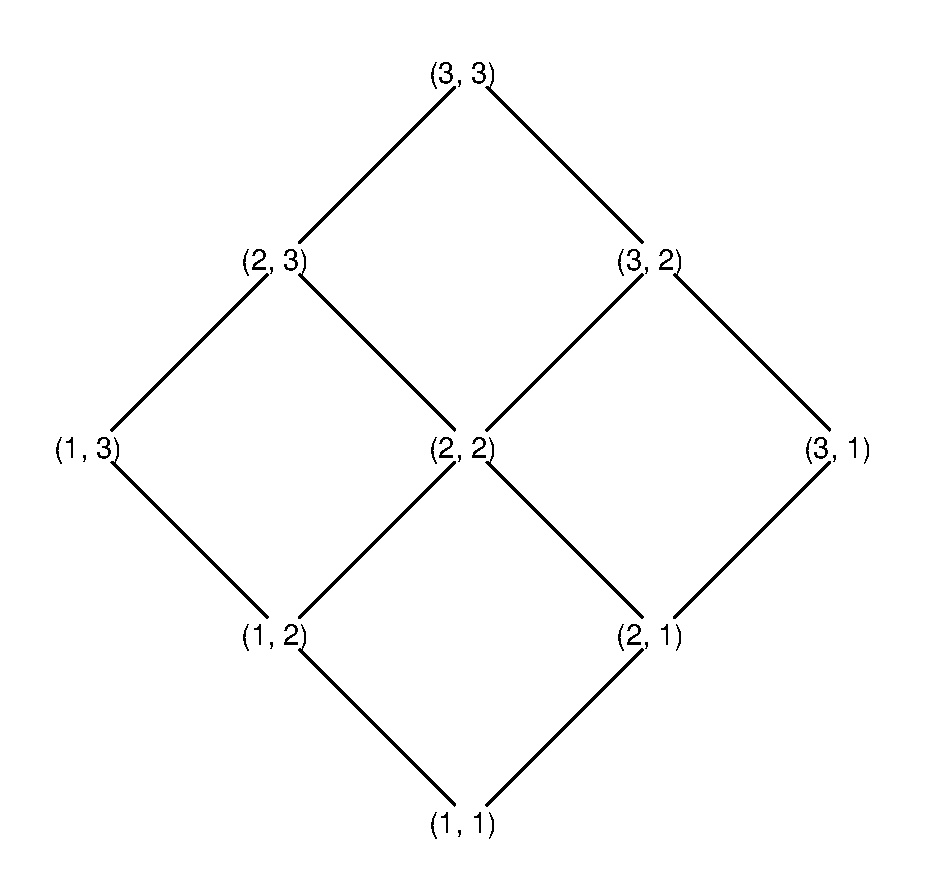
\includegraphics[width=13cm]{aufgabe1a-hasse}
%\caption{This is a figure.}
\end{center}
\end{figure}

\subsection*{b)}
Gegeben zwei Elemente $(x_1, y_1) \in \mathbb{N}^+ \times \mathbb{N}^+ $ und
$(x_2, y_2) \in \mathbb{N}^+ \times \mathbb{N}^+ $ kann das Infimum mit folgender Funktion berechnet werden:

\begin{align*}
&inf:  (\mathbb{N}^+ \times \mathbb{N}^+) \times  (\mathbb{N}^+ \times \mathbb{N}^+)  \to \mathbb{N}^+ \times \mathbb{N}^+ \\
&((x_1, y_1), (x_2, y_2))  \mapsto (min(x_1, x_2), min(y_1, y_2))
\end{align*}

Das Supremum berechnet diese Funktion:
\begin{align*}
&sup:  (\mathbb{N}^+ \times \mathbb{N}^+) \times  (\mathbb{N}^+ \times \mathbb{N}^+)  \to \mathbb{N}^+ \times \mathbb{N}^+ \\
&((x_1, y_1), (x_2, y_2))  \mapsto (max(x_1, x_2), max(y_1, y_2))
\end{align*}

\subsection*{c)}
Sei $ X \subseteq  \mathbb{N}^+ \times \mathbb{N}^+ $ und $ x \in X$. Dann lässt sich das Infimum mit folgender Funktion berechnen:
\begin{align*}
& \Inf : X \to x \\
& \Inf (X) = (min(\{x \medspace | \medspace \exists y. (x, y) \in X\}),
min(\{y \medspace| \medspace\exists x. (x, y) \in X\})
% TODO: abstände um | schöner machen
\end{align*}

Das Supremum berechnet diese Funktion:
\begin{align*}
& \Sup : X \to x \\
& \Sup (X) = (max(\{x \medspace| \medspace\exists y. (x, y) \in X\}),
max(\{y \medspace| \medspace\exists x. (x, y) \in X\})
% TODO: Abstände
\end{align*}
Für unendliche Teilmengen $X$ ist die Funktion undefiniert, da dann $max$ kein größtes Element finden kann.

\subsection*{d)}

\begin{align*}
& \bot = (0, 0)
\end{align*}
$\top $ existiert nicht, da die Trägermenge $ \mathbb{N}^+ \times \mathbb{N}^+ $ das Kreuzprodukt der natürlichen Zahlen ist.
Da $\mathbb{N} $ unendlich ist und kein größtes Element besitzt, gibt es auch in $ \mathbb{N}^+ \times \mathbb{N}^+ $ kein größtes Element.

\subsection*{e)}
$V$ ist ein Verband, da die Funktionen aus Aufgabenteil b) für jede zweielementige
 Teilmenge von $V$ das Infimum und das Supremum berechnen können.
Allerdings ist $V$ kein vollständiger Verband, da die Funktion $\Sup$ aus
Aufgabenteil c) für unendliche Teilmengen der Trägermenge undefiniert ist.
Das heißt es existiert nicht für alle Teilmengen der Trägermenge von $V$
 ein Supremum und somit kann $V$ kein vollständiger Verband sein.

\subsection*{f)}
Zu zeigen: Für alle $(x_1, y_1), (x_2, y_2) \in \mathbb{N}^+ \times \mathbb{N}^+ $ gilt: \\
$ (x_1, y_1) \leq_2 (x_2, y_2) \Rightarrow f((x_1, y_1)) \leq_2 f((x_2, y_2))$ \\
Seien $g$ und $h$ Funktionen: \\

\begin{align*}
& g: \mathbb{N}^+ \to  \mathbb{N}^+\\
&  g(x) = x! \\
& h: \mathbb{N}^+ \to  \mathbb{N}^+\\
&  h(y) = 2y^2 +2y -1 \\
\end{align*}
Es gilt offensichtlich:
\begin{align*}
& f((x, y)) = (h(y), g(x))
\end{align*}
Seien $ (x_1, y_1), (x_2, y_2) \in \mathbb{N}^+ \times \mathbb{N}^+ $
 mit $ (x_1, y_1) \leq_2 (x_2, y_2) $.
Dann gilt:

\begin{align}
& f((x_1, y_1)) = (h(y_1), g(x_1))
\end{align}

Es gilt außerdem:

\begin{align}
& f((x_2, y_2)) = (h(y_2), g(x_2))
\end{align}

Um die Prämisse zu erfüllen muss gelten:
\begin{align*}
& f((x_1, y_1)) \leq_2 f((x_2, y_2)) \\
\end{align*}
Aus (1) und (2) folgt, das folgendes ebenso gelten muss \\
\begin{align*}
& \Leftrightarrow (h(y_1), g(x_1)) \leq_2 (h(y_2), g(x_2)) \\
\end{align*}
Aus der Definition von  $\leq_2 $ folgt, dass dazu gelten muss: \\
\begin{align*}
& \Leftrightarrow h(y_1) \leq h(y_2) \land  g(x_1) \leq g(x_2) \\
\end{align*}

Betrachte beide Voraussetzungen getrennt: \\
1. Zu zeigen: $ h(y_1) \leq h(y_2) $ \\
Das gilt mit $y_1 \leq y_2$ immer, wenn $h$ monoton ist. \\
Dazu muss gelten: $h(n) \leq h (n+1), n \in \mathbb{N}^+$ \\
\begin{align*}
 h(n) &= 2n^2+2n-1 &\\
&\leq 2n^2 +6n +3 = 2n^2 +4n +2 +2n +2 -1 & n > 0\\
& = 2(n+1)^2 + 2(n+1) -1 = h(n+1) &\\
\end{align*}
Also ist $h$ monoton und die erste Voraussetzung gilt.

2. Zu zeigen: $g(x_1) \leq g(x_2) $ \\
Das gilt unter der gegebenen Voraussetzung $ x_1 \leq x_2 $ immer,
wenn $g$ monoton ist. \\
Dazu muss gelten: $g(n) \leq g(n+1), n \in \mathbb{N}^+ $ \\
\begin{align*}
g(n) &= n! &\\
&\leq (n+1) * n! & n > 0\\
& =(n+1)!= g(n+1)&
\end{align*}
Also ist auch $g$ monoton und die zweite Voraussetzung gilt ebenso.\\

Aus der Gültigkeit beider Voraussetzungen folgt, dass auch $f$ monoton ist.\\
$\Box$



%Das gilt mit $y_1 \leq y_2$ immer, wenn h monoton ist. \\
%Beweis der Monotonie von h per vollständige Induktion:\\
%Induktionsbehauptung: $\forall n \in \mathbb{N}^+. h(n) \leq h(n+1)$ \\
%Induktionsanfang $n = 1$ \\
%$ h(n) = h(1) = 2 + 2 -1 = 3 $\\
%$ h (n +1) = h(2) = 8 + 4 -1 = 11 $\\
%Damit gilt die IB für ein $ n \in \mathbb{N}$.\\
%Induktionsvoraussetzung: Es gilt $h(n) \leq h(n+1)$ \\
%Induktionsschritt: Betrachte $ n+1$ \\
%Zu zeigen: $ h(n+1) \leq h(n+1+1) $\\
%$ h(n+1) = 2(n+1)^2 + 2(n+1) -1 $ \\
%$ = 2(n+1)^2 +2n + 2 -1 = 2(n+1)^2 + 2n + 1 $\\
%$ = 2(n^2 + 2n + 1) + 2n + 1 $ \\
%$ = 2n^2 + 4n + 2+ 2n +1 $ \\
%$ = 2n^2 + 6n +3 $\\
%Mit $ n > 0 $und der IV gilt: \\
%$ \le 2n^2 + 10n + 11 $ \\
%$ = 2n^2 + 8n +8 + 2n + 4 -1 $ \\
%$ = 2(n^2 +4n+4) + 2n +4 -1 $ \\
%$= 2(n+2)^2 + 2(n+2) -1$\\
%$ = h( n + 2) = h(n+1+1)$ \\
%Somit gilt die Induktionsbehautung für ein $ n $ sowie $(n+1)$,
% also für alle $n \in \mathbb{N}^+$.
%
%
%
%2. Zu zeigen: $ g(x_1) \leq g(x_2) $\\
%Das gilt mit $ x_1 \leq x_2$ immer, wenn g monoton ist.\\
%TODO: Beweis der Monotonie von g (vollst. Induktion)
%
%Somit gelten beide Voraussetzungen und damit ist auch f monoton.\\
%$\Box $

\subsection*{Aufgabe 2 - Rekursive Eigenschaften}

\subsubsection*{a)}

$ F = \poss{anmelden} Even( \poss{pruefen} \necess{\Act} \false)$ \\

Explizit: \\

\begin{align*}
Y =& \poss{anmelden} X \\
X \HMmin& \poss{pruefen}\necess{ \Act } \false \lor (\poss{ \Act } \true \land \necess { \Act } X )
\end{align*}


\subsubsection*{b)}

$ F = Inv(Poss(\poss{gewinnen} \true))$ \\

Explizit: \\

\begin{align*}
Y \HMmin& \poss{gewinnen} \true \lor \poss{ \Act } Y \\
X \HMmax& Y \land \necess{ \Act } X
\end{align*}

\subsubsection*{c)}

$ F = Inv(\poss{pruefen} \true) \mathcal{U}^s \poss{durchfallen} \necess{pruefen} \false$ \\

Explizit: \\

\begin{align*}
Y \HMmax& \poss{pruefen} \true \land \poss{ \Act } Y \\
X \HMmin& \poss{durchfallen} \land \necess{\Act  \setminus \{durchfallen\}} \false \lor
(Y \land \poss{\Act} \true \land \necess{\Act}X)
\end{align*}


\subsection*{Aufgabe 3 - Charakteristische Formeln}

\subsubsection*{a)}

\begin{align*}
X_1 \HMmax& \necess{ \Act } \false \\
X_2 \HMmax& \poss{b} X_1 \land \necess{a}\false \land \necess{c}\false \land \necess{b}X_1 \\
X_3 \HMmax& \poss{a}X_5 \land \poss{b}X_7 \land \poss{c}X_6 \land \necess{a}X_5 \land \necess{b}X_7 \land \necess{c}X_6 \\
X_4 \HMmax& \poss{b}X_1 \land \poss{b}X_9 \land \necess{a}\false \land \necess{c}\false \land \necess{b}(X_1 \lor X_9) \\
X_5 \HMmax& \poss{a}X_2 \land \poss{a}X_4 \land \necess{b}\false \land \necess{c}\false \land \necess{a}(X_2 \lor X_4) \\
X_6 \HMmax& \poss{a}X_8 \land \necess{b}\false \land \necess{c}\false \land \necess{a}X_8 \\
X_7 \HMmax& \poss{a}X_8 \land \necess{b}\false \land \necess{c}\false \land \necess{a}X_8 = X_6\\
X_8 \HMmax& \poss{b}X_9 \land \necess{a}\false \land \necess{c}\false \land \necess{b}X_9 \\
X_9 \HMmax& \necess{ \Act } \false \\
\end{align*}

\subsubsection*{b)}

Es existieren die folgenden Äquivalenzklassen: \\

\begin{align*}
\necess{1}_\sim =& \{ 1, 9\} \\
\necess{3}_\sim =& \{ 3\} \\
\necess{5}_\sim =& \{ 5, 6, 7\} \\
\necess{2}_\sim =& \{ 2, 4, 8\} \\
\end{align*}

%\section*{Aufgabe 4: Bisimulation (2)}

$\mathcal{F}^{1}(Proc \times Proc) = r(s(\{(R_1, R_7),(R_2, R_4),(R_2, R_6),(R_3, R_5),(R_4, R_6),(R_8, R_9)\}))$
\\
$\mathcal{F}^{2}(Proc \times Proc) = r(s(\{(R_2, R_6),(R_3, R_5)\}))$
\\
$\mathcal{F}^{3}(Proc \times Proc) = r(s(\{(R_2, R_6),(R_3, R_5)\})) = \mathcal{F}^{2}$
\\\\
Da $\mathcal{F}^{2} = \mathcal{F}^{3}$ sind beide ein Fixpunkt.
\\
Somit erhalten wir, dass $R_2$ und $R_6$ sowie $R_3$ und $R_5$ die einzigen nicht trivialen bisimilaren Paare sind. Es gilt $R_2$ \bisim $R_6$ und $R_3$ \bisim $R_5$.

\section*{Aufgabe 5: Starke Bisimulation}

\subsection*{d)}

Sei $\mathcal{B} = \{(q_2, p_1),(q_1, p_2),(q_4,p_2),(q_3,p_4),(q_5,p_3)\}$. \\
Beweis, dass $\mathcal{B} $ eine starke Bisimulation ist:

\begin{compactitem}
\item \ShowBisim{\MC{B}}{p_1,q_2}{{a, p_2, q_4}}{{a, q_4, p_2}}
\item \ShowBisim{\MC{B}}{q_1,p_2}{{c,q_3,p_4},{b,q_5,p_3}}{{b, p_3,q_5},{c, p_4,q_3}}
\item \ShowBisim{\MC{B}}{q_4,p_2}{{b,q_5,p_3}}{{b, p_3,q_5}}
\item \ShowBisim{\MC{B}}{q_3,p_4}{{a,q_5,p_3}}{{a, p_3,q_5}}
\item \ShowBisim{\MC{B}}{q_5,p_3}{{a,q_2,p_1}}{{a, p_1, q_2}}
\end{compactitem}

Da $\mathcal{B}$ eine starke Bisimulation ist und $(q_2, p_1) \in \mathcal{B}$, gilt $q_2 \bisim p_1$.
\subsection*{a), b), c)}
Da $q_2 \bisim p_1$ (Beweis siehe d), gilt auch, dass $ q_2$ von $  p_1$ stark simuliert wird, sowie dass $p_1 $ von $ q_2$ stark simuliert wird. Damit simulieren sich $q_2$ und $p_2$ auch stark gegenseitig.

\documentclass[11pt]{paper}

%\usepackage[T1]{fontenc}
\usepackage[utf8]{inputenc}
\usepackage[ngerman]{babel}
%\usepackage[]{}


\begin{document}

\end{document}
\section*{Aufgabe 7: Schwache Bisimulation}

\subsection*{a)}
Zu zeigen: $i \wbisim j$

Sei $\MC{B} = \{(i,j),(i_1,j_1),(i_2,j_1),(i_1,j_3),(i_1,j_4),(i_3,j_3),(i,j_2),(i_4,j_3),(i_4,j_4)\}$. \\
Zu zeigen: $\MC{B}$ ist eine schwache Bisimulation.

\begin{compactitem}
\item \ShowBisim{\MC{B}}{i,j}{{a,i_1,j_1},{a,i_2,j_1}}{{a,j_1,i_1}}
\item \ShowBisim{\MC{B}}{i_1,j_1}{{b,i_1,j_3},{c,i_1,j_4}}{{\tau,j_3,i_1}}
\item \ShowBisim{\MC{B}}{i_2,j_1}{{\tau,i_3,j_3},{d,i,j_2}}{{\tau,j_3,i_1},{d,j_2,i}}
\item \ShowBisim{\MC{B}}{i_1,j_3}{{b,i_1,j_3},{c,i_1,j_4}}{}
\item \ShowBisim{\MC{B}}{i_1,j_4}{{b,i_1,j_3},{c,i_1,j_3}}{}
\item \ShowBisim{\MC{B}}{i_3,j_3}{{b,i_4,j_3},{c,i_3,j_4}}{{b,j_3,i_4},{c,j_4,i_3}}
\item \ShowBisim{\MC{B}}{i,j_2}{{a,i_2,j_1},{a,i_1,j_1}}{{\tau,j,i}}
\item \ShowBisim{\MC{B}}{i_4,j_3}{{c,i_4,j_4},{b,i_3,j_3}}{{c,j_4,i_4},{b,j_3,i_3}}
\item \ShowBisim{\MC{B}}{i_4,j_4}{{b,i_3,j_3},{c,i_4,j_3}}{{c,j_3,i_4},{b,j_3,i_3}}
\end{compactitem}
Somit ist $\MC{B}$ eine schwache Bisimulation. Da $(i, j) \in \MC{B}$ kann gefolgert werden, dass $i$ und $j$ schwach bisimilar sind.

\subsection*{b)} $i \not\approx k$, weil in $k$ auch nach der ersten c-Aktion noch eine d-Aktion möglich ist, in $i$ aber nach dem ersten c kein Weg mehr zu einer d-Aktion exisitiert.

\subsection*{c)} $j \not\approx k$, weil in $k$ auch nach der ersten c-Aktion noch eine d-Aktion möglich ist, in $i$ aber nach dem ersten c kein Weg mehr zu einer d-Aktion exisitiert.


\end{document}
